\documentclass[crop,tikz]{standalone}

\begin{document}
  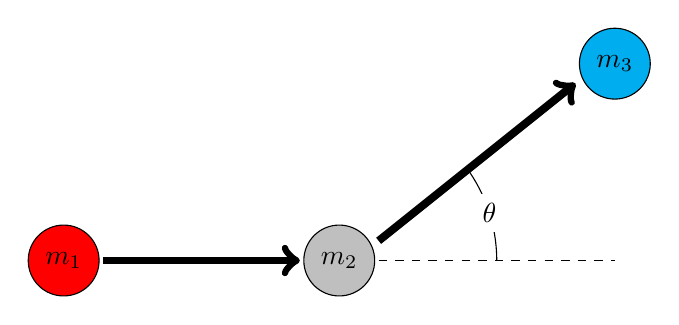
\begin{tikzpicture}
    \node[circle, draw, fill=red, minimum size = 0.9cm] (c) at (-3.5,0){$m_1$}; 
    \draw [-to, line width=1mm] (-3,0) -- (-0.5,0);
    \node[circle, draw, fill=lightgray, minimum size = 0.9cm] (c) at (0,0){$m_2$}; 
    \node[circle, draw, fill=cyan, minimum size = 0.9cm] (c) at (3.5, 2.5){$m_3$}; 
    \draw [-to, line width=1mm] (0.5,0.25) -- (3,2.25);
    \draw [dashed] (0.5,0) -- (3.5,0);
    \draw (2,0) arc [start angle=0, end angle=35, x radius=2cm, y radius =2cm] node[midway,fill=white] {$\theta$};
  \end{tikzpicture}
\end{document}